\documentclass[aspectratio=169,9pt]{beamer}

\usepackage[utf8]{inputenc}
\usepackage[T1]{fontenc}
\usepackage{lmodern}
\usepackage[brazilian]{babel}
\usepackage{booktabs}
\usepackage{graphicx}
\usepackage{amsmath}
\usepackage{appendixnumberbeamer}
\graphicspath{{../fig/metodologia/}{figuras/}} % figuras da monografia, sem cópia, e figuras só dos slides

\usetheme{Madrid}
\usecolortheme{default}
\setbeamertemplate{navigation symbols}{}
\setbeamertemplate{footline}[frame number]
 

\title[Eleições e finanças municipais]{O Efeito das Eleições nas Finanças Municipais:\\Evidências Empíricas para os Municípios Brasileiros}
\author[Lorenzo Rodrigues Geronazzo]{Lorenzo Rodrigues Geronazzo\texorpdfstring{\\[0.4em]}{, }{\small Orientador: Prof.~Dr.~Victor Rodrigues de Oliveira}}
\institute{Universidade Federal do Paraná\\Curso de Ciências Econômicas}
\date{25 de novembro de 2026}

\begin{document}


%--------------------------------------------------
% TÍTULO
%--------------------------------------------------
\begin{frame}
  \titlepage
  
\end{frame}

%--------------------------------------------------
% 1. GANCHO (1 min)
%--------------------------------------------------
\begin{frame}[plain]
  \vfill
  \begin{center}
    {\Huge \textbf{R\$ 93,8 bilhões}}\\[1em]
    {\Large de impacto direto nas contas públicas em 2026}\\[0.6em]
    {\normalsize gastos e isenções de impostos do governo federal, sem contar linhas de crédito}\\[1.5em]
    {\large Ano de eleição presidencial.}\\[1.5em]
    {\Large \textit{Políticas voltadas ao bem-estar da população\\ ou oportunismo eleitoral?}}
  \end{center}
  \vfill
  {\tiny Fonte: cálculo da Instituição Fiscal Independente (IFI/Senado Federal), divulgado pela CNN Brasil em 16 out. 2026.}
\end{frame}
\note{(1 min) Apresente o número e faça a pergunta. Composição (IFI, via CNN Brasil): R\$ 63,2 bi em despesas primárias e R\$ 30,6 bi em renúncias fiscais. Somando crédito subsidiado (R\$ 185,7 bi) e recursos fora do orçamento (R\$ 18,9 bi), o total mobilizado chega a R\$ 298,4 bi. O cálculo inclui medidas de todo o mandato, como a isenção do IR, e os subsídios aos combustíveis adotados por causa da guerra no Oriente Médio; no segundo semestre vieram o Desenrola 3.0, o reajuste do Bolsa Família e o fim das bets. O governo nega caráter eleitoral. Leve à pergunta de pesquisa: este trabalho faz a mesma pergunta para os municípios, com dados.}

%--------------------------------------------------
% 2. PROBLEMA E HIPÓTESES (1,5 min)
%--------------------------------------------------
\begin{frame}{Problema de pesquisa e hipóteses}
  \textbf{Pergunta:} de que forma o calendário eleitoral e o alinhamento político do prefeito com o governador e com o presidente afetam o \alert{volume} e a \alert{composição} das despesas dos municípios brasileiros (2013--2025)?
  \vspace{1em}
  \begin{block}{H1 --- Ciclo eleitoral}
    No ano eleitoral, há recomposição do orçamento em favor das despesas mais visíveis ao eleitor (obras urbanas, transporte, saúde), em detrimento das menos visíveis (administração).
  \end{block}
  \begin{block}{H2 --- Alinhamento político}
    O alinhamento do prefeito com o governador e com o presidente está associado a maior despesa, via transferências voluntárias.
  \end{block}
\end{frame}
\note{(1,5 min) Apresente a pergunta e as duas hipóteses. Mencione os objetivos específicos só de passagem.}

%--------------------------------------------------
% 3. REFERENCIAL TEÓRICO (2 min)
%--------------------------------------------------
\begin{frame}{Referencial teórico: três explicações para o ciclo}
  \begin{description}
    \item[Nordhaus (1975)] Ciclo \alert{oportunista}: o governante expande a atividade antes da eleição e eleitores míopes o recompensam.
    \item[Rogoff (1990)] \alert{Sinalização}: eleitores racionais; o governante usa gastos de rápida percepção para sinalizar competência.
    \item[Drazen e Eslava (2010)] \alert{Recomposição}: o ciclo ocorre mesmo sem déficit, deslocando gasto para itens mais visíveis ao eleitor.
  \end{description}
  \vspace{1em}
  \begin{alertblock}{Hipótese testada neste trabalho}
    Recomposição em favor das despesas visíveis (Drazen e Eslava, 2010).
  \end{alertblock}
\end{frame}
\note{(2 min) Linha do tempo da teoria. Destaque Drazen e Eslava, que é a hipótese que você testa. Se perguntarem, Hibbs e Alesina são a vertente partidária.}

%--------------------------------------------------
% 4. EVIDÊNCIA PARA O BRASIL E LACUNA (1,5 min)
%--------------------------------------------------
\begin{frame}{Evidência para o Brasil e lacuna}
  \begin{itemize}
    \item \textbf{Sakurai (2009)}, 1990--2005: o ano eleitoral eleva o gasto em Saúde e Saneamento, Habitação e Urbanismo e Transporte.
    \item \textbf{Ferreira e Bugarin (2007)}: municípios cujo prefeito é da coligação do governador, ou do partido do presidente, recebem mais transferências voluntárias.
  \end{itemize}
  \vspace{0.5em}
  \textbf{O que mudou desde então:}
  \begin{itemize}
    \item contas padronizadas no Siconfi;
    \item recessão de 2014--2016;
    \item pandemia coincidindo com a eleição de 2020;
    \item mudanças bruscas na coalizão do governo federal.
  \end{itemize}
  \vspace{0.5em}
  \alert{Contribuição:} atualizar a evidência para 2013--2025, com quase todos os municípios do país e a classificação funcional atual.
\end{frame}
\note{(1,5 min) Apresente a lacuna e a contribuição.}

%--------------------------------------------------
% 5. DADOS (1,5 min)
%--------------------------------------------------
\begin{frame}{Dados}
  \begin{columns}[T]
    \begin{column}{0.5\textwidth}
      \begin{itemize}
        \item Painel de \textbf{5.569 municípios}, 2013--2025
        \item \textbf{71.307} observações município-ano
        \item Despesa \textbf{paga}, por função (Siconfi/DCA)
        \item Valores em R\$ de 2025, per capita
      \end{itemize}
    \end{column}
    \begin{column}{0.5\textwidth}
      \textbf{Fontes}
      \begin{itemize}
        \item STN (Siconfi): despesas e receitas
        \item TSE: prefeitos, governadores, presidente, coligações
        \item IBGE: população, PIB, Censo
      \end{itemize}
    \end{column}
  \end{columns}
  \vspace{1em}
  \textbf{Variáveis dependentes (9):} despesa total e oito grupos de funções (Saúde e Saneamento, Educação e Cultura, Habitação e Urbanismo, Assistência Social, Transporte, Administração, Agricultura, Comunicações).
\end{frame}
\note{(1,5 min) Seja breve. Os agrupamentos seguem Sakurai (2009), com dois ajustes: Assistência Social sem Previdência e inclusão de Administração como contraste.}

%--------------------------------------------------
% 6. ESTRATÉGIA EMPÍRICA (2 min)
%--------------------------------------------------
\begin{frame}{Estratégia empírica: dois modelos de efeitos fixos}
  \begin{block}{Modelo A --- ciclo eleitoral}
    \[
      \ln(1+d_{it}^{k}) = \beta_1\,\text{Eleitoral}_t + \beta_2\,\text{PréEleitoral}_t + \beta_3\,\text{Pandemia}_t + \dots + c_i + u_{it}
    \]
    Efeito fixo de município; erros-padrão de Driscoll e Kraay.
  \end{block}
  \begin{block}{Modelo B --- alinhamento político}
    \[
      \ln(1+d_{it}^{k}) = \gamma_1\,\text{CoalGov}_{it} + \gamma_2\,\text{CoalPres}_{it} + \dots + c_i + \tau_t + u_{it}
    \]
    Efeitos fixos de município e de ano: compara prefeitos alinhados e não alinhados \alert{no mesmo ano}.
  \end{block}
  \small
  \begin{itemize}
    \item Hausman rejeita efeitos aleatórios nas nove variáveis.
    \item Log: coeficientes lidos como variação percentual.
    \item Efeito fixo de ano necessário: prefeitos alinhados ao presidente passam de 59\% (2015--18) a 1\% (2019--22).
  \end{itemize}
\end{frame}
\note{(2 min) Driscoll-Kraay: ``protege contra choques nacionais comuns a todos os municípios''. Sem efeito fixo de ano, o alinhamento com o presidente se confunde com o período (0,9\% sem ele, nulo com ele).}

%--------------------------------------------------
% EVIDÊNCIA DESCRITIVA: DESPESA TOTAL (0,5 min)
%--------------------------------------------------
\begin{frame}{Evidência descritiva: despesa total}
  \begin{center}
    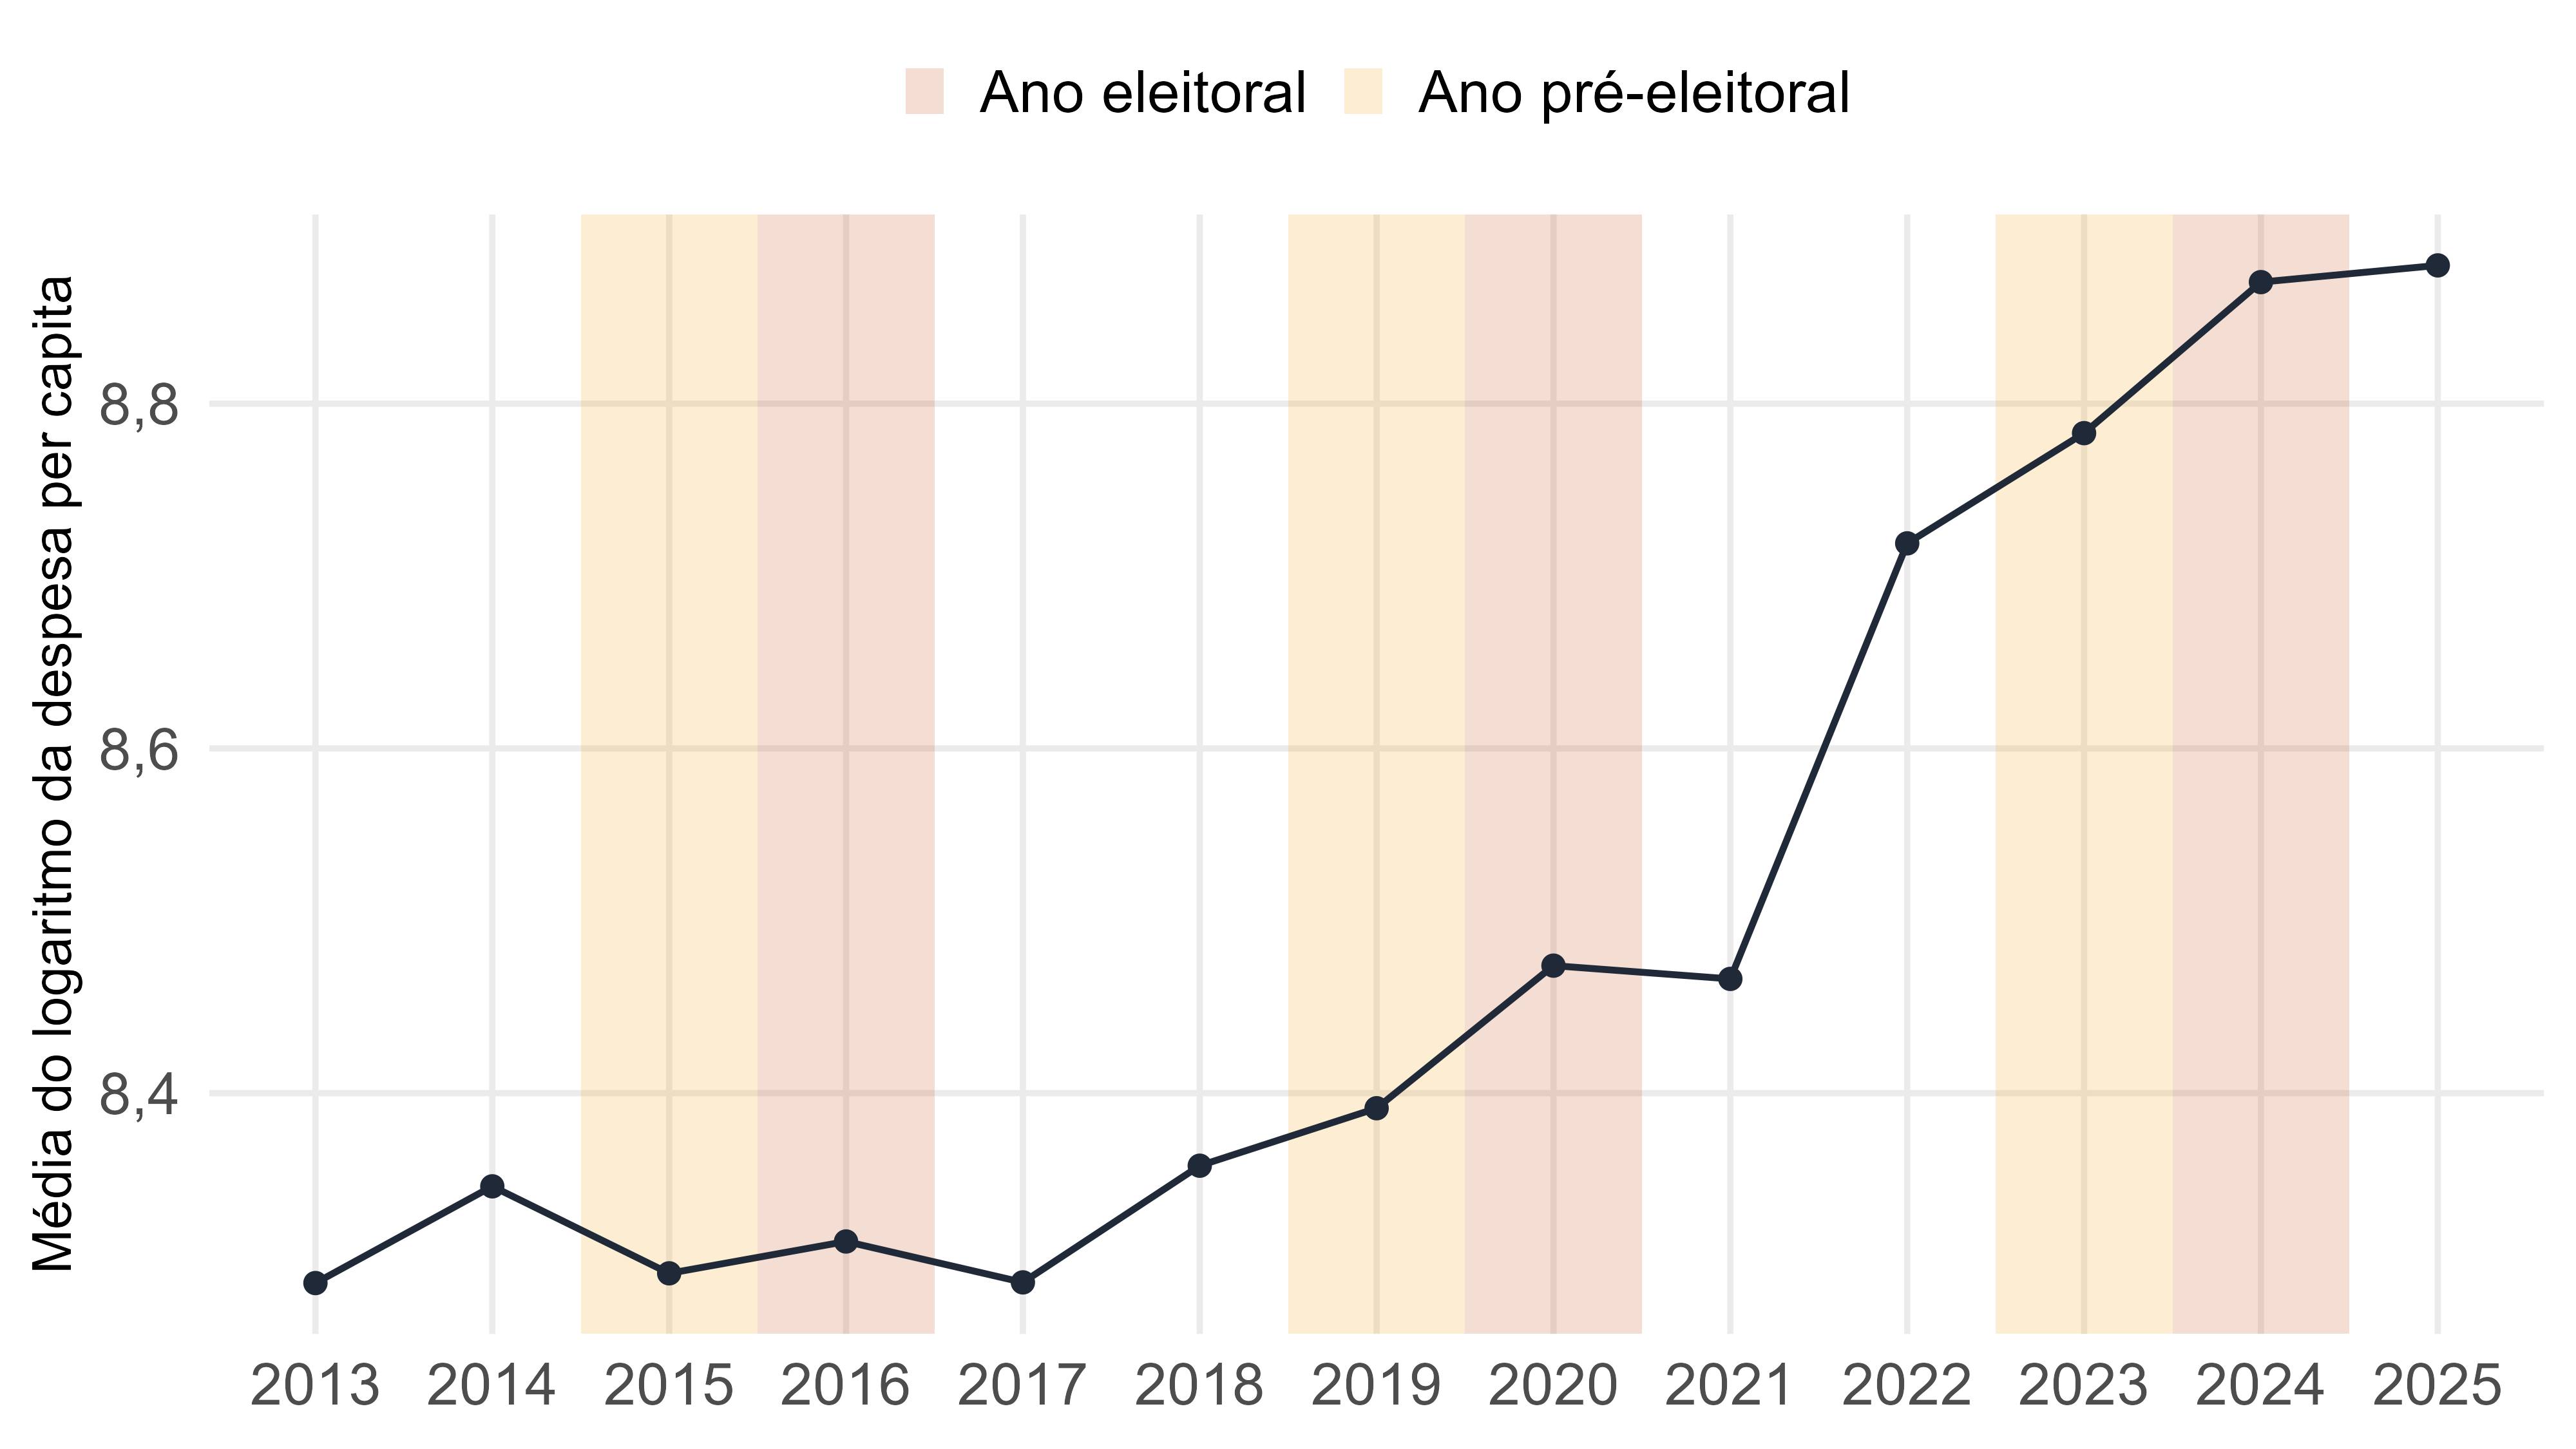
\includegraphics[width=\textwidth,height=0.75\textheight,keepaspectratio]{figuras/serie_despesa_total_slides.png}
  \end{center}
  \vspace{0.5em}
  \small Na despesa total, a tendência de alta domina, e os anos eleitorais quase não se destacam.
\end{frame}
\note{(0,5 min) Mostre que o total cresce de forma contínua. O contraste com o próximo slide é o ponto: o ciclo aparece nos itens visíveis.}

%--------------------------------------------------
% 7. EVIDÊNCIA DESCRITIVA (1 min)
%--------------------------------------------------
\begin{frame}{Evidência descritiva: Habitação e Urbanismo e Transporte}
  \begin{center}
    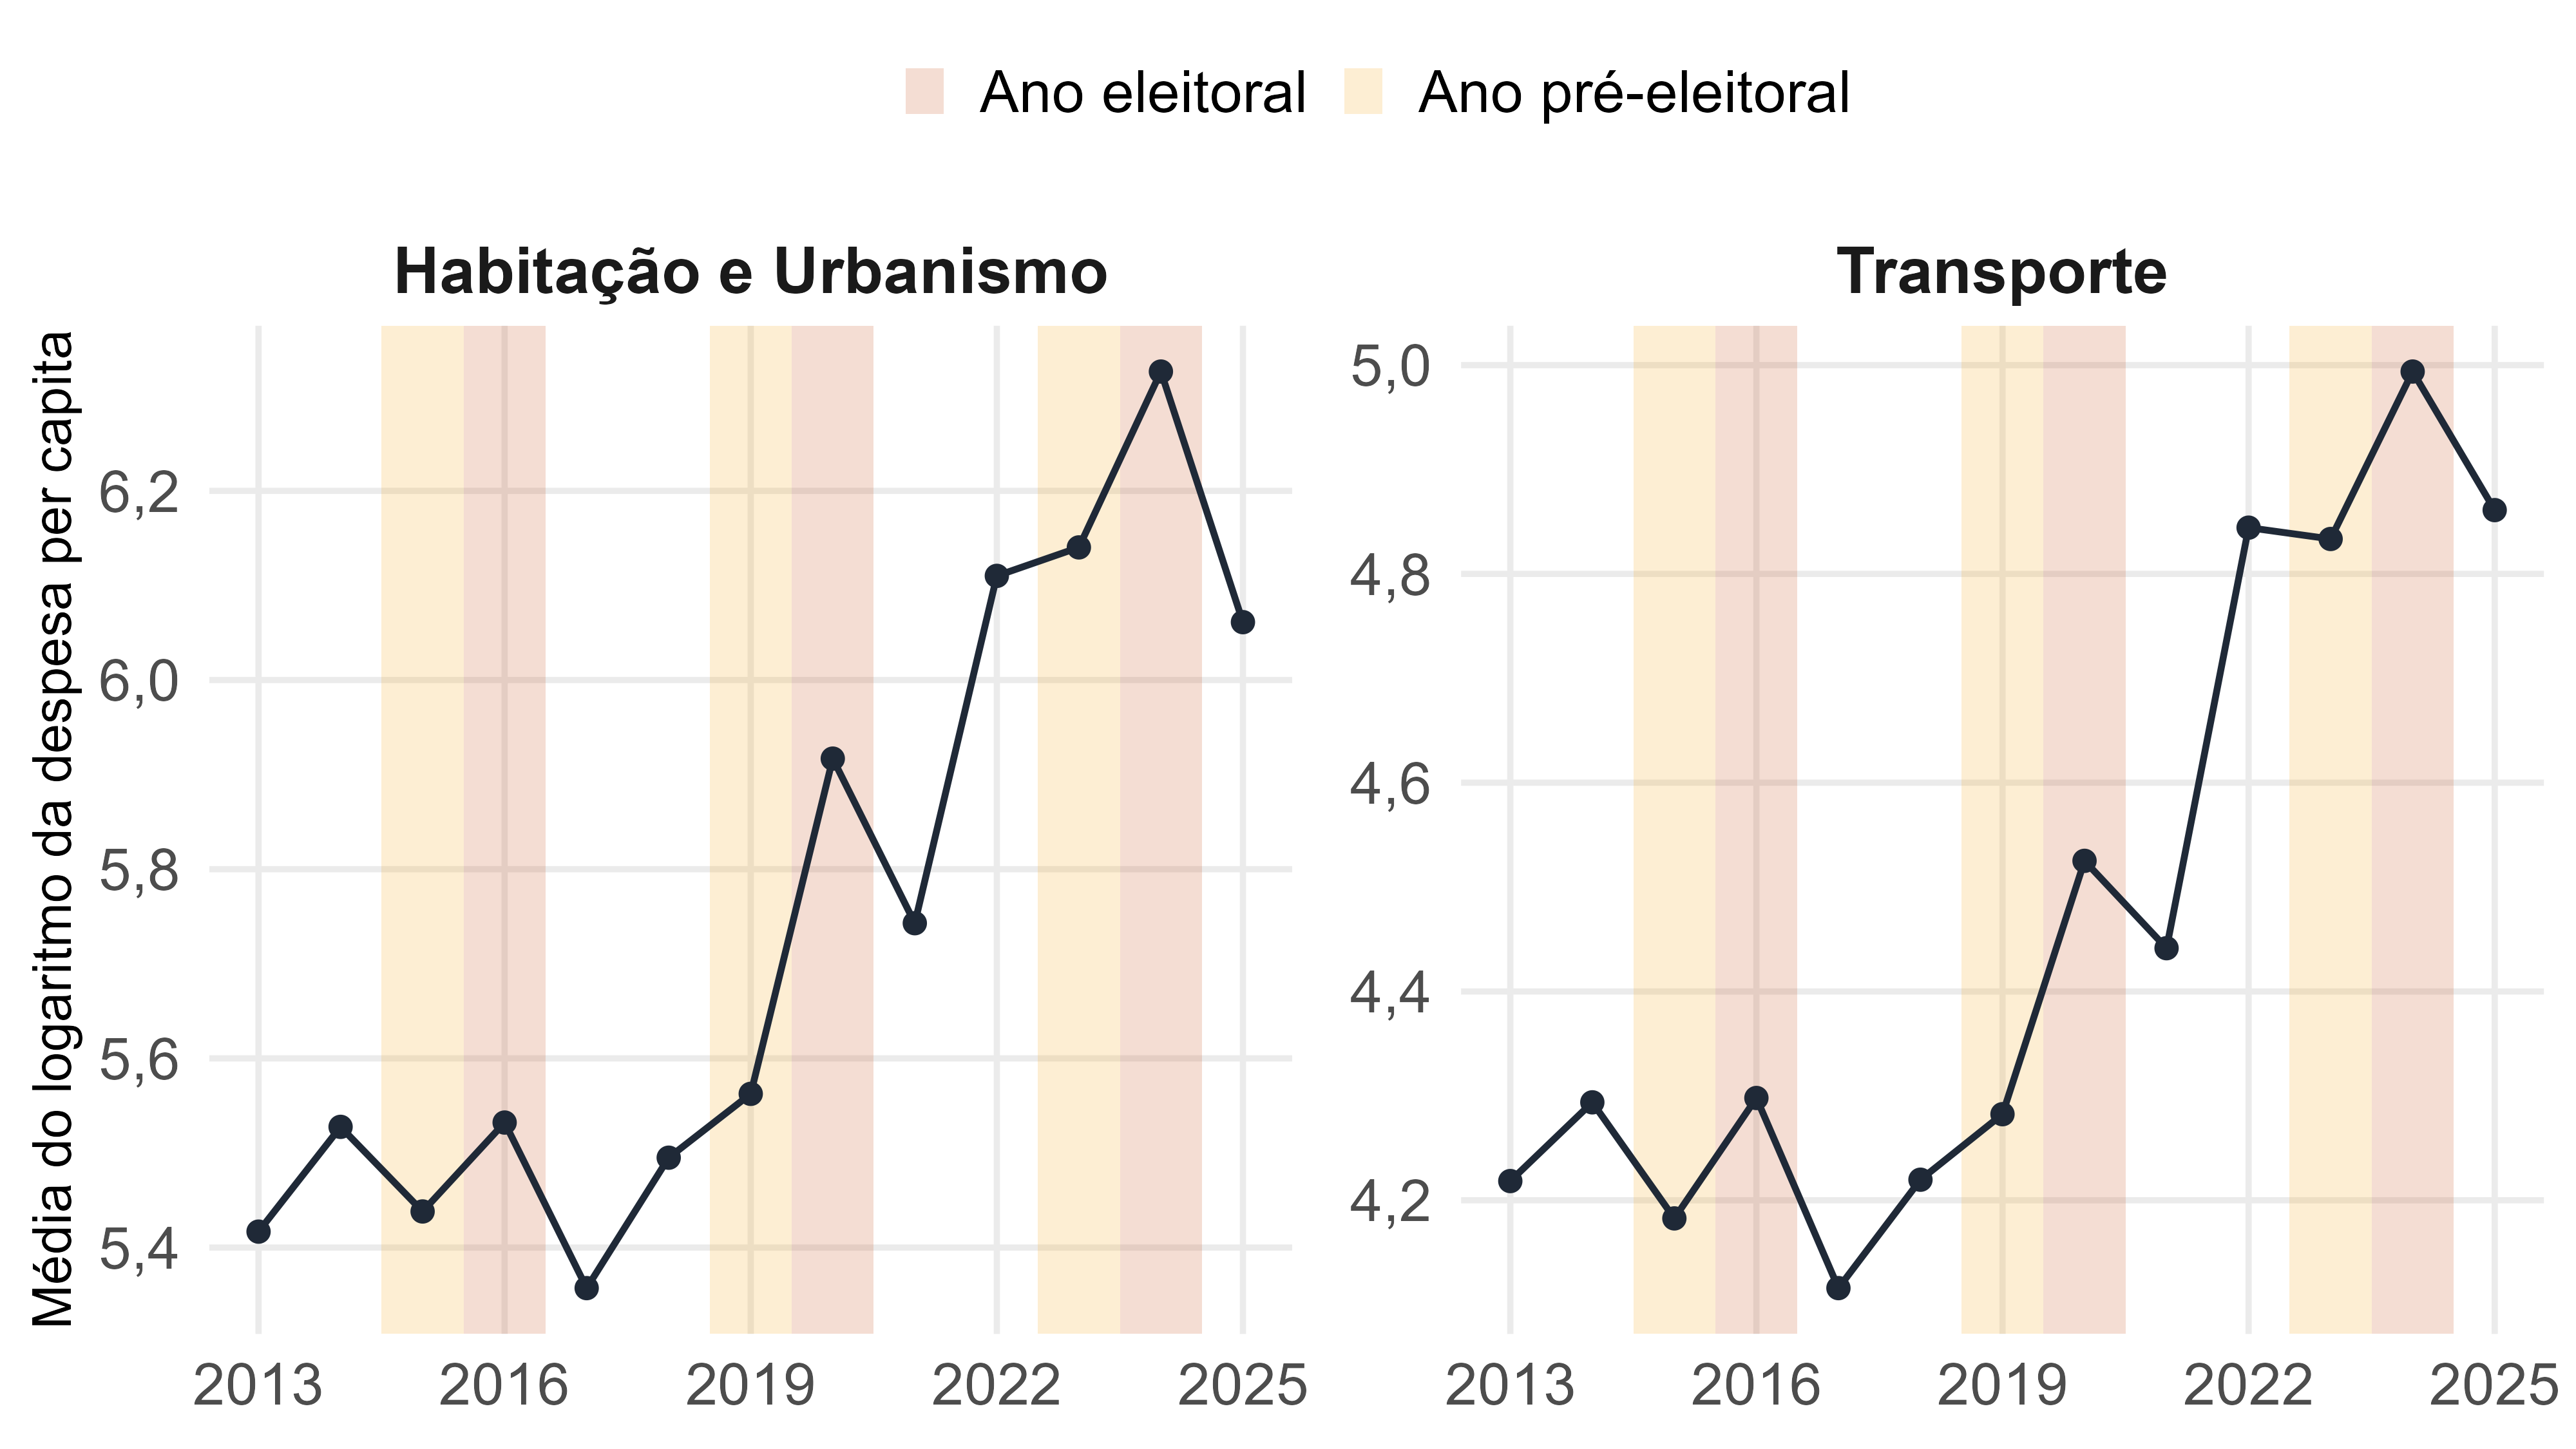
\includegraphics[width=\textwidth,height=0.80\textheight,keepaspectratio]{grupos_slides_A.png}
  \end{center}
\end{frame}
\note{(0,5 min) Os dois maiores efeitos do trabalho. Mostre os picos nos anos eleitorais (faixas vermelhas).}

\begin{frame}{Evidência descritiva: Saúde e Saneamento e Assistência Social}
  \begin{center}
    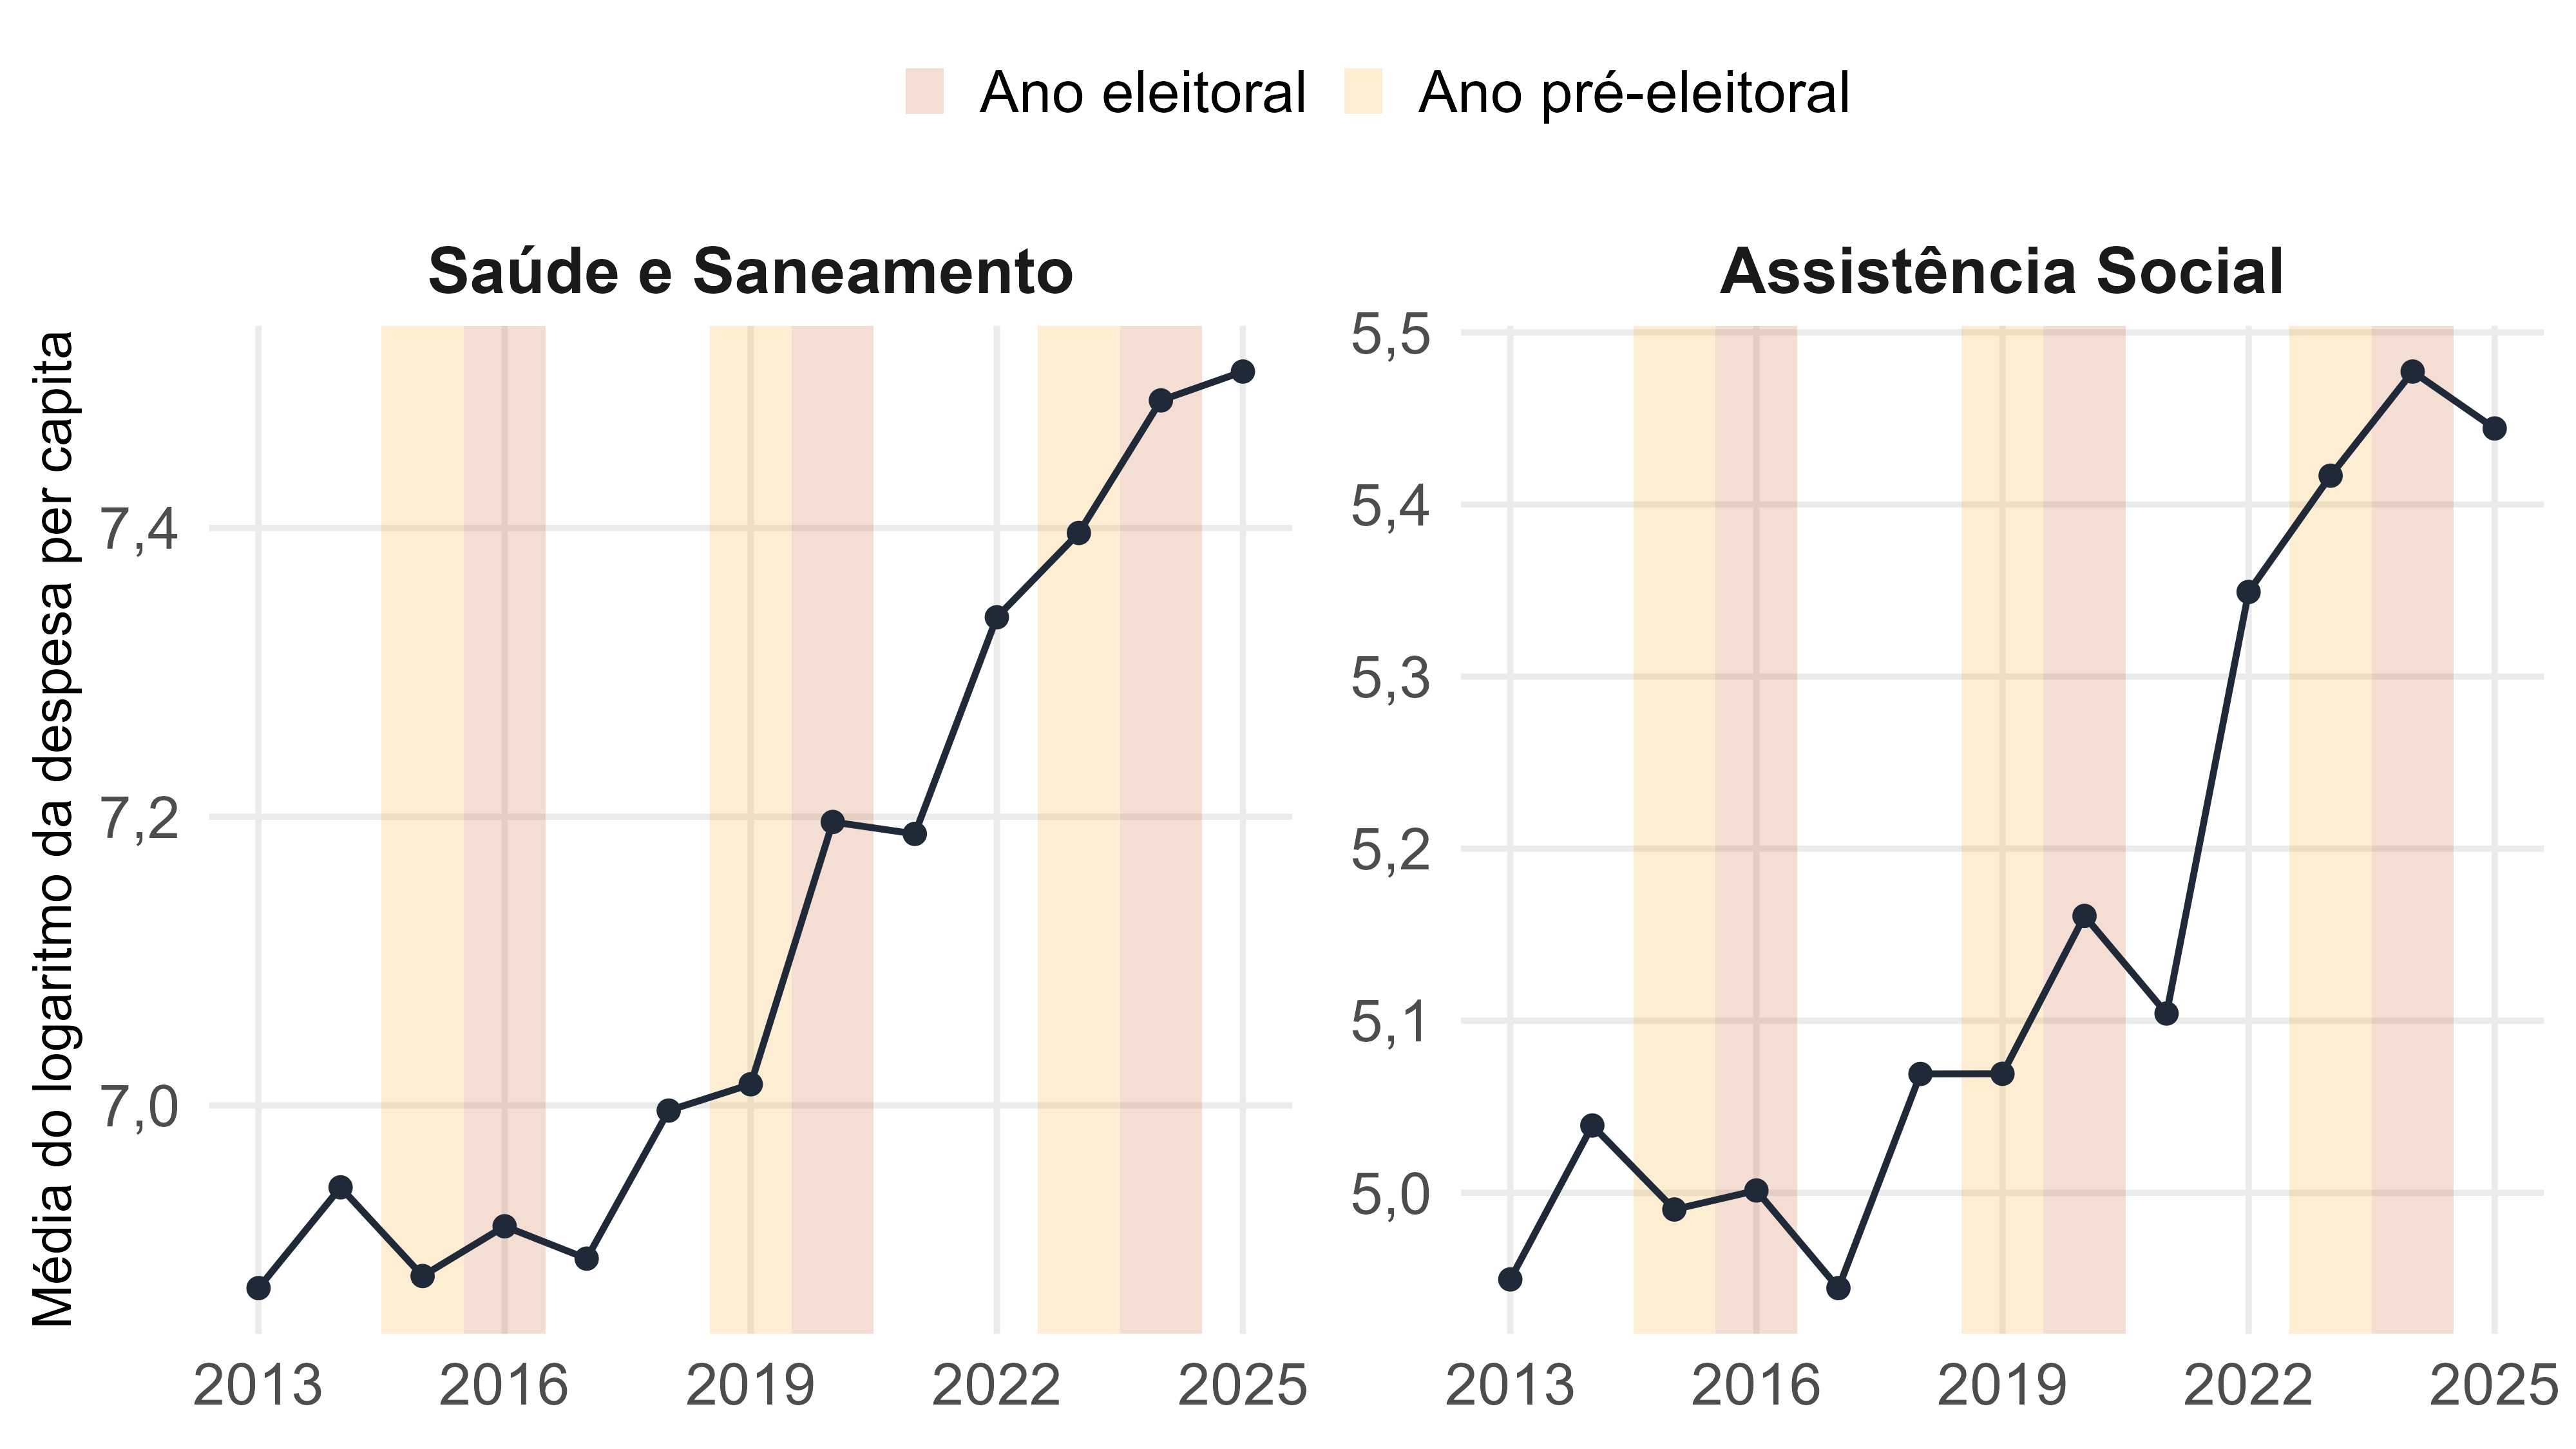
\includegraphics[width=\textwidth,height=0.75\textheight,keepaspectratio]{grupos_slides_B.png}
  \end{center}
  \vspace{0.5em}
  \small O gráfico \alert{sugere}, mas não separa a eleição de outros choques (pandemia em 2020; aumento das receitas a partir de 2022).
\end{frame}
\note{(1 min) Seja honesto: a leitura gráfica motiva a análise econométrica, que controla receitas, demografia, PIB e tendência.}

%--------------------------------------------------
% 8. RESULTADO 1 (2 min)
%--------------------------------------------------
\begin{frame}{Resultado 1: o ciclo se concentra no que é visível}
  \begin{center}
    \begin{tabular}{lcccl}
      \toprule
      \textbf{Função (ano eleitoral)} & \textbf{Média} & \textbf{2016} & \textbf{2024} & \textbf{Leitura}\\
      \midrule
      Habitação e Urbanismo & $+27\%$     & $+24\%$     & $+28{,}7\%$ & sólido \\
      Transporte            & $+19{,}5\%$ & $+21{,}2\%$ & $+17{,}6\%$ & sólido (cautela na magnitude) \\
      Saúde e Saneamento    & $+4{,}2\%$  & $+4{,}2\%$  & $+4\%$      & sólido \\
      Assistência Social    & $+7\%$      & n.s.        & $+9{,}1\%$  & só em 2024 \\
      Administração         & n.s.        & n.s.        & $+2{,}2\%$  & só em 2024 \\
      \midrule
      \textbf{Despesa total} & {\boldmath$+5{,}3\%$} & $+3{,}3\%$ & $+6{,}7\%$ & 2016 sensível à especificação \\
      \bottomrule
    \end{tabular}
  \end{center}
  \vspace{0.3em}
  \begin{itemize}
    \item Em 2024 quase tudo sobe, inclusive Administração: boom de receitas ou estratégia eleitoral? O desenho não separa as duas.
  \end{itemize}
  \vfill
  {\scriptsize Modelo A; despesa per capita em logaritmo. Média: 2016 e 2024 (2020 absorvido pela \textit{dummy} de pandemia). n.s.: não significativo.}
\end{frame}
\note{(2 min) É o slide principal. ``Sólido'' = significativo com os dois erros-padrão, nas duas eleições e nas duas formas funcionais (log e nível). Com a amostra até 2023, o efeito de 2016 sobre a despesa total perde significância na especificação principal (R7a).}

%--------------------------------------------------
% 10. RESULTADO 3 (1 min)
%--------------------------------------------------
\begin{frame}{Resultado 2: recomposição das participações}
  \begin{center}
    \begin{tabular}{lc}
      \toprule
      \textbf{Participação na despesa total} & \textbf{Ano eleitoral (p.p.)} \\
      \midrule
      Habitação e Urbanismo & $+1{,}46$ \\
      Transporte            & $+0{,}44$ \\
      Assistência Social    & $+0{,}06$ \\
      Saúde e Saneamento    & n.s. \\
      Agricultura           & n.s. \\
      Administração         & $-0{,}45$ \\
      Educação e Cultura    & $-0{,}55$ \\
      \bottomrule
    \end{tabular}
  \end{center}
  {\scriptsize Modelo A (teste R4); variável dependente: participação na despesa total (\%). n.s.: não significativo. Comunicações não é interpretada (valores muito pequenos).\par}
  \vspace{0.5em}
  \alert{Expansão concentrada nos itens visíveis, com recomposição} --- e não a troca pura sem aumento do total prevista por Drazen e Eslava (2010).
\end{frame}
\note{(1 min) Saúde e Saneamento cresce em proporção semelhante à do total, por isso não muda de participação.}

%--------------------------------------------------
% 11. RESULTADO 4 (1,5 min)
%--------------------------------------------------
\begin{frame}{Resultado 3: alinhamento político}
  \begin{columns}[T,onlytextwidth]
    \begin{column}{0.48\textwidth}
      \begin{block}{Governador}
        Despesa total \alert{$\approx +0{,}4\%$}: efeito pequeno, mas estável em todos os testes.\\[0.5em]
        Administração: $\approx +0{,}7\%$.
      \end{block}
    \end{column}
    \hfill
    \begin{column}{0.48\textwidth}
      \begin{block}{Presidente}
        \alert{Sem efeito} na despesa total (amostra completa).\\[0.5em]
        Medida com erro: só 1,2\% dos prefeitos aparecem alinhados em 2019--22.
      \end{block}
    \end{column}
  \end{columns}
  \vspace{1em}
  \textbf{Atenção:} são \alert{associações}, não efeitos causais; o alinhamento muda quando mudam o prefeito, o governador ou o presidente.
\end{frame}
\note{(1,5 min) A coalizão do governo de 2019--22 com o Centrão (PP, PL) não aparece na variável, que usa só a coligação vencedora da eleição presidencial. Prefeitos do PP e do PL governavam cerca de 19\% dos municípios em 2021--22.}

%--------------------------------------------------
% 12. ROBUSTEZ E LIMITAÇÕES (1,5 min)
%--------------------------------------------------
\begin{frame}{Robustez e limitações}
  \textbf{18 testes de robustez.}
  \vspace{0.5em}
  \begin{columns}[T]
    \begin{column}{0.5\textwidth}
      \textbf{O que resiste}
      \begin{itemize}
        \item Habitação, Transporte e Saúde no ano eleitoral
        \item Nas duas eleições, nas duas formas funcionais, com os dois erros-padrão
        \item Alinhamento com o governador na despesa total
      \end{itemize}
    \end{column}
    \begin{column}{0.5\textwidth}
      \textbf{O que não resiste}
      \begin{itemize}
        \item Educação e Cultura (depende do tratamento de 2020)
        \item Agricultura (depende da forma funcional)
        \item Efeito de 2016 na despesa total (amostra até 2023)
      \end{itemize}
    \end{column}
  \end{columns}
  \vspace{0.5em}
  \textbf{Limitações:} apenas duas eleições identificam o efeito; despesa medida no estágio do pagamento; sem separação entre custeio e investimento.
\end{frame}
\note{(1,5 min) Assuma as ressalvas antes de a banca perguntar.}

%--------------------------------------------------
% 13. CONCLUSÃO E AGENDA (1 min)
%--------------------------------------------------
\begin{frame}{Conclusão e agenda futura}
  \begin{itemize}
    \item O ciclo eleitoral municipal é uma \alert{expansão concentrada nos itens mais visíveis}: Habitação e Urbanismo ($+27\%$), Transporte ($+19{,}5\%$) e Saúde e Saneamento ($+4{,}2\%$).
    \item Confirma, para o período recente, parte dos achados de Sakurai (2009).
    \item Alinhamento com o governador: efeito pequeno, mas estável.
  \end{itemize}
  \vspace{0.5em}
  \textbf{Próximos passos}
  \begin{itemize}
    \item Estágios de empenho e restos a pagar
    \item Classificação por natureza (custeio $\times$ investimento)
    \item Transferências voluntárias e de capital
    \item Eleições seguintes
  \end{itemize}
  \vspace{0.5em}
  \alert{Volta ao gancho:} nos municípios, o gasto do ano eleitoral se concentra no que o eleitor vê --- o padrão que a teoria associa ao oportunismo e à sinalização.
\end{frame}
\note{(1 min) Feche voltando ao dado de abertura.}

%--------------------------------------------------
% OBRIGADO
%--------------------------------------------------
\begin{frame}[plain,noframenumbering]
  \vfill
  \begin{center}
    {\Huge Obrigado!}\\[1em]
    {\Large Perguntas?}
  \end{center}
  \vfill
\end{frame}

%==================================================
% SLIDES DE RESERVA
%==================================================
\appendix

\begin{frame}{Reserva A --- Modelo A (resumo)}
  \begin{center}
    \small
    \begin{tabular}{lcccc}
      \toprule
       & \textbf{Desp.\ total} & \textbf{Saúde e San.} & \textbf{Habitação} & \textbf{Transporte}\\
      \midrule
      Ano eleitoral    & 0,0519*** & 0,0411*** & 0,2389*** & 0,1778*** \\
      Ano pré-eleitoral & 0,0209   & $-0{,}0083$ & 0,0509** & 0,0188 \\
      Pandemia (2020)  & $-0{,}0058$ & 0,0908*** & 0,1254*** & 0,0711*** \\
      \bottomrule
    \end{tabular}
  \end{center}
  {\scriptsize Efeito fixo de município; erros-padrão de Driscoll-Kraay. *** $p<0{,}01$; ** $p<0{,}05$. Ver Tabela 6 da monografia.}
\end{frame}

\begin{frame}{Reserva B --- Testes de robustez selecionados}
  \begin{itemize}
    \item \textbf{R3:} especificação em nível (despesa total: R\$ 277,87 per capita, cerca de 5\% da média)
    \item \textbf{R5:} especificação de Sakurai (2009)
    \item \textbf{R7 e R7a:} amostra 2013--2023 (alinhamento com o presidente fica negativo, $\approx -0{,}3\%$)
    \item \textbf{R12:} erro-padrão agrupado por município
    \item \textbf{R14:} sem a dummy de pandemia (Educação e Cultura perde significância)
    \item \textbf{R17:} população interpolada em 2022 e 2023
  \end{itemize}
\end{frame}

\begin{frame}{Reserva C --- Pandemia e mudança de base da população}
  \begin{itemize}
    \item 2020 é, ao mesmo tempo, ano eleitoral e ano de pandemia: a dummy de pandemia faz o efeito eleitoral ser identificado por 2016 e 2024.
    \item Em 2020: Saúde e Saneamento $\approx +9{,}5\%$ e Educação e Cultura $\approx -14{,}9\%$.
    \item A série oficial de população muda de base em 2022 (Censo), o que afeta os valores per capita de 2022 e 2023. O teste R17 mostra que isso não altera os resultados principais.
  \end{itemize}
\end{frame}

\begin{frame}{Reserva D --- Mecanismos específicos do Brasil}
  \begin{itemize}
    \item \textbf{Federalismo fiscal:} transferências voluntárias não são neutras (Ferreira e Bugarin, 2007).
    \item \textbf{Interação espacial:} spillover e yardstick competition (Videira e Mattos, 2011).
    \item \textbf{Restos a pagar:} uso estratégico de restos a pagar não processados no ano eleitoral (Vicente e Nascimento, 2012).
    \item \textbf{LRF:} restringe a expansão direta de gastos e desloca os incentivos para manobras contábeis.
  \end{itemize}
\end{frame}

\end{document}